\documentclass[11pt,a4paper]{article}

\usepackage[margin=2.0cm,top=2.2cm,bottom=2.2cm]{geometry}
\usepackage{amsmath,amssymb}
\usepackage{booktabs}
\usepackage{array}
\usepackage{tabularx}
\usepackage{graphicx}
\usepackage{float}
\usepackage[table]{xcolor}
\usepackage{enumitem}
\usepackage{caption}
\usepackage{fancyhdr}
\usepackage{hyperref}
\usepackage{xeCJK}

\setCJKmainfont[Path=/System/Library/Fonts/Supplemental/,AutoFakeBold=2.2,AutoFakeSlant=0.15]{Arial Unicode.ttf}
\setCJKsansfont[Path=/System/Library/Fonts/,AutoFakeBold=2.0]{STHeiti Medium.ttc}
\setCJKmonofont[Path=/System/Library/Fonts/]{STHeiti Light.ttc}

\renewcommand{\figurename}{图}
\renewcommand{\tablename}{表}

\definecolor{PrimaryBlue}{HTML}{1F4E79}
\definecolor{AccentRed}{HTML}{B02A2A}
\definecolor{SoftBg}{HTML}{F4F7FA}
\definecolor{BorderGray}{HTML}{CBD5E1}

\hypersetup{
  colorlinks=true,
  linkcolor=PrimaryBlue,
  urlcolor=PrimaryBlue,
  citecolor=PrimaryBlue,
  pdftitle={LIBERO-RSI-Bench Imitation Learning (ACT) Experimental Report},
  pdfauthor={libero-rsi-bench}
}

\captionsetup{font=small,labelfont=bf}

\pagestyle{fancy}
\fancyhf{}
\fancyhead[L]{\small\color{gray} LIBERO-RSI-Bench — 模仿学习基线实验报告}
\fancyhead[R]{\small\color{gray} Dual-Camera ACT (\texttt{il\_act\_50} vs. \texttt{il\_act\_20})}
\fancyfoot[C]{\small\thepage}
\renewcommand{\headrulewidth}{0.4pt}

\graphicspath{{figures/}}

\title{\vspace{-1.0cm}\textbf{\Large \textsf{LIBERO-RSI-Bench：模仿学习 (Dual-Camera ACT) 完整基准实验报告}}\\[0.35em]
\large \textsf{Full-Data (\texttt{il\_act\_50}) 与 Low-Data (\texttt{il\_act\_20}) 域内/域外消融评测、失败聚类及双视角闭环仿真分析}}
\author{\textsf{实验平台：AutoDL NVIDIA GeForce RTX 5090 (32\,GB VRAM, \texttt{MuJoCo 2.3.7 + LIBERO-plus})}}
\date{\textsf{2026 年 11 月 23 日}}

\begin{document}
\maketitle
\vspace{-0.4cm}

\begin{center}
\fcolorbox{BorderGray}{SoftBg}{%
\begin{minipage}{0.95\textwidth}
\small
\textbf{核心结论摘要（624 条闭环仿真轨迹全量实测）：}
\begin{itemize}[leftmargin=1.4em,itemsep=2pt,topsep=2pt]
  \item \textbf{全量基线 (\texttt{il\_act\_50}, 165 demos, 0.901\,GPUh)}：在域内盲测集 \texttt{TEST\_ID} ($N=100$) 上达到 \textbf{SR@1.0x = 90.0\% / SR@1.5x = 91.0\%}（95\% Wilson CI: \texttt{[83.8\%, 95.2\%]}），在 4 轴域外抗干扰盲测集 \texttt{TEST\_OOD} ($N=112$) 上达到 \textbf{SR@1.0x = 78.6\% / SR@1.5x = 79.5\%}（\texttt{[71.1\%, 85.9\%]}）。
  \item \textbf{低数据消融 (\texttt{il\_act\_20}, 80 demos, 0.485\,GPUh)}：数据量减半后，\texttt{TEST\_ID} 仅轻微下降 4.0 个百分点至 \textbf{87.0\% / 87.0\%}（配对 Exact McNemar $p=0.3877$，域内差异不显著）；但 \texttt{TEST\_OOD} 显著跌至 \textbf{67.9\% / 68.8\%}（全量组胜出 $+10.7\%$，Exact McNemar \textbf{$p=0.0169 < 0.05$}）。
  \item \textbf{结构性短板定位}：纯视觉模仿学习在语义改写（\texttt{language\_instruction}: 100.0\%）与桌面局部布局扰动（\texttt{objects\_layout}: 96.4\%）上极强，但在 \textbf{相机视觉外参扰动 (\texttt{camera\_visual}: 60.7\% / 42.9\%)}、\textbf{机械臂初始状态偏移 (\texttt{robot\_init\_state}: 60.7\% / 53.6\%)} 以及 \textbf{长时序双阶段任务 (\texttt{long\_t0}: 68.0\% / 60.0\% ID)} 上表现薄弱，为后续与 RSI (Code-as-Policies) 对比提供了精准对照基线。
\end{itemize}
\end{minipage}}
\end{center}

\section{实验背景与统一基准协议}

为与后续 \textbf{RSI (Recursive Self-Improvement / Code-as-Policies)} 方法在同一仿真动力学、观测契约、动作空间、步数预算与四维成本口径下进行严格公平对比，本实验严格遵循 \texttt{docs/BENCHMARK\_SPEC.md} 与锁定盲测切分文件 \texttt{protocol/splits.lock.json}（SHA-256 前缀 \texttt{792b1a0dee9acd25...}）。

\subsection{核心任务集与双视野预算 (Dual-Horizon Protocol)}

基准测试覆盖 \texttt{LIBERO} 与 \texttt{sylvestf/LIBERO-plus} 的 4 个代表性操作任务，每个任务均锁定标准步数上限 ($1.0\times$) 与 1.5 倍扩展步数上限 ($1.5\times$)：

\begin{table}[H]
\centering
\caption{四大核心基础操作任务及其步数预算定义}
\label{tab:tasks}
\small
\begin{tabular}{@{}llp{5.5cm}cc@{}}
\toprule
\textbf{任务代号} & \textbf{所属套件} & \textbf{标准语言指令} & \textbf{标准上限 ($1.0\times$)} & \textbf{扩展上限 ($1.5\times$)} \\
\midrule
\texttt{spatial\_t0} & \texttt{libero\_spatial} & pick up the black bowl between the plate and the ramekin and place it on the plate & 220 steps & 450 steps \\
\texttt{object\_t0} & \texttt{libero\_object} & pick up the alphabet soup and place it in the basket & 280 steps & 450 steps \\
\texttt{goal\_t0} & \texttt{libero\_goal} & open the middle drawer of the cabinet & 300 steps & 450 steps \\
\texttt{long\_t0} & \texttt{libero\_10} & put both the alphabet soup and the tomato sauce in the basket & 520 steps & 750 steps \\
\bottomrule
\end{tabular}
\end{table}

\subsection{三大锁定切分集与四维成本账本}

\begin{itemize}[leftmargin=1.5em,itemsep=2pt]
  \item \textbf{\texttt{DEV} 开发集（$N=100$）}：4 任务各 25 条域内演示初始状态，用于超参数校验与闭环一致性检查。
  \item \textbf{\texttt{TEST\_ID} 域内盲测集（\texttt{sealed\_id}, $N=100$）}：与训练同分布的保留初始状态（各 25 条），通过 \texttt{--confirm-unseal} 解封并记录于 \texttt{runs/sealed\_reads.log}。
  \item \textbf{\texttt{TEST\_OOD} 域外盲测集（\texttt{sealed\_ood}, $N=112$）}：基于 \texttt{LIBERO-plus} 映射 4 大域外扰动轴（\texttt{objects\_layout} 物体布局与干扰物、\texttt{robot\_init\_state} 机械臂初始关节角偏移、\texttt{language\_instruction} 指令同义改写、\texttt{camera\_visual} 相机视角与背景材质视觉扰动），每轴 28 条、每任务 28 条。
  \item \textbf{四维生命周期成本账本 (\texttt{CostLedger})}：严格统计离线演示条数 (\texttt{demo\_count})、在线交互回合 (\texttt{online\_episodes})、训练算力 (\texttt{gpu\_hours}) 与推理大语言模型消耗 (\texttt{total\_tokens})，并遵守协议上限（每任务 $\le 50$ 条演示、$\le 100$ Epochs、0 在线训练回合）。
\end{itemize}

\section{模仿学习策略架构与训练流水线}

\subsection{Dual-Camera Action Chunking Transformer (ACT) 架构}

策略网络在 \texttt{baselines/il\_policy.py}（\texttt{ILChunkingPolicy} / \texttt{ActionChunkingTransformer}）中实现，直接消耗纯像素双视角观测与本体状态，不接触任何真值物体状态或场景图：
\begin{enumerate}[leftmargin=1.6em,itemsep=2pt]
  \item \textbf{双视角空间软特征编码}：\texttt{agentview}（第三人称全局相机）与 \texttt{robot0\_eye\_in\_hand}（腕部第一人称相机）原始 $256\times 256$ RGB 图像先经 180° 旋转对齐 \texttt{LeRobot/LIBERO} 标准视野，下采样至 $128\times 128$ 后分别输入独立的 \texttt{ResNet-18} 骨干网，并通过 \texttt{SpatialSoftmax2d(4x4)} 提取 $512\times 2$ 维空间关键点坐标后投影至 $d=256$ 视觉 Token。
  \item \textbf{本体状态与任务条件嵌入}：8D 本体状态向量 \texttt{[eef\_pos(3), axisangle(3), gripper\_qpos(2)]} 经 Z-score 标准化后由 2 层 MLP 映射至 $d=256$ Token；语言指令通过 \texttt{infer\_task\_idx()} 关键词锚点解析（兼容 \texttt{language\_instruction} OOD 同义改写）索引可学习任务嵌入 \texttt{task\_emb(8, 256)}。
  \item \textbf{动作分块解码与时序平滑}：将 \texttt{[tok\_task, tok\_state, tok\_agent, tok\_wrist]} 与 $C=16$ 个可学习查询位姿 \texttt{query\_pos} 拼接为 20 个序列 Token，经 4 层 8 头 \texttt{TransformerEncoder}（\texttt{norm\_first=True}, \texttt{GELU}, \texttt{dropout=0.1}）联合交互后输出 $16\times 7$ 动作块（7D \texttt{osc\_delta\_eef}：6D 末端位姿增量裁剪至 $[-1,1]$ + 二值夹爪指令 $\{-1, +1\}$）。闭环评测时启用步长为 16 窗口的指数衰减时序平滑（Temporal Ensembling，$k=0.01$）。
\end{enumerate}

\subsection{专家数据提取与 RTX 5090 100-Epoch 训练收敛}

通过 \texttt{protocol/hf\_matched\_shards.json} 对 \texttt{HuggingFaceVLA/libero}（共 377 个 Parquet 分片）精确探测出覆盖上述 4 个任务的 146 个分片，使用 \texttt{baselines/prepare\_dataset.py} 提取共计 \textbf{165 条}专家轨迹（\texttt{spatial\_t0}: 45 条 / 4,487 帧；\texttt{object\_t0}: 44 条 / 6,867 帧；\texttt{goal\_t0}: 43 条 / 6,019 帧；\texttt{long\_t0}: 33 条 / 9,571 帧；总计 26,944 帧）。在训练阶段施加随机裁剪偏移与色彩抖动增广以增强 OOD 视觉鲁棒性，并在单卡 \textbf{NVIDIA GeForce RTX 5090 (Blackwell \texttt{sm\_120})} 上完成两个对比模型训练（均使用 \texttt{AdamW} 配合 100-Epoch 余弦退火学习率从 $2\times 10^{-4}$ 降至 $1\times 10^{-6}$）：
\begin{itemize}[leftmargin=1.5em,itemsep=2pt]
  \item \textbf{\texttt{il\_act\_50}}：165 条轨迹（26,944 帧），39,100 梯度步（$<50\text{k}$ 协议上限），训练 Smooth-L1 损失从 Epoch 1 的 \texttt{0.5622} 稳步收敛至 Epoch 100 的 \textbf{\texttt{0.0518}}，总训练耗时 \textbf{\texttt{0.901 GPUh}}（约 54 分钟）。
  \item \textbf{\texttt{il\_act\_20}}：每任务截取前 20 条轨迹，共 80 条轨迹（13,687 帧，占全量帧数的 50.8\%），20,400 梯度步，训练损失从 \texttt{0.6578} 收敛至 Epoch 100 的 \textbf{\texttt{0.0535}}，总训练耗时 \textbf{\texttt{0.485 GPUh}}（约 29 分钟）。
\end{itemize}

\begin{figure}[H]
\centering
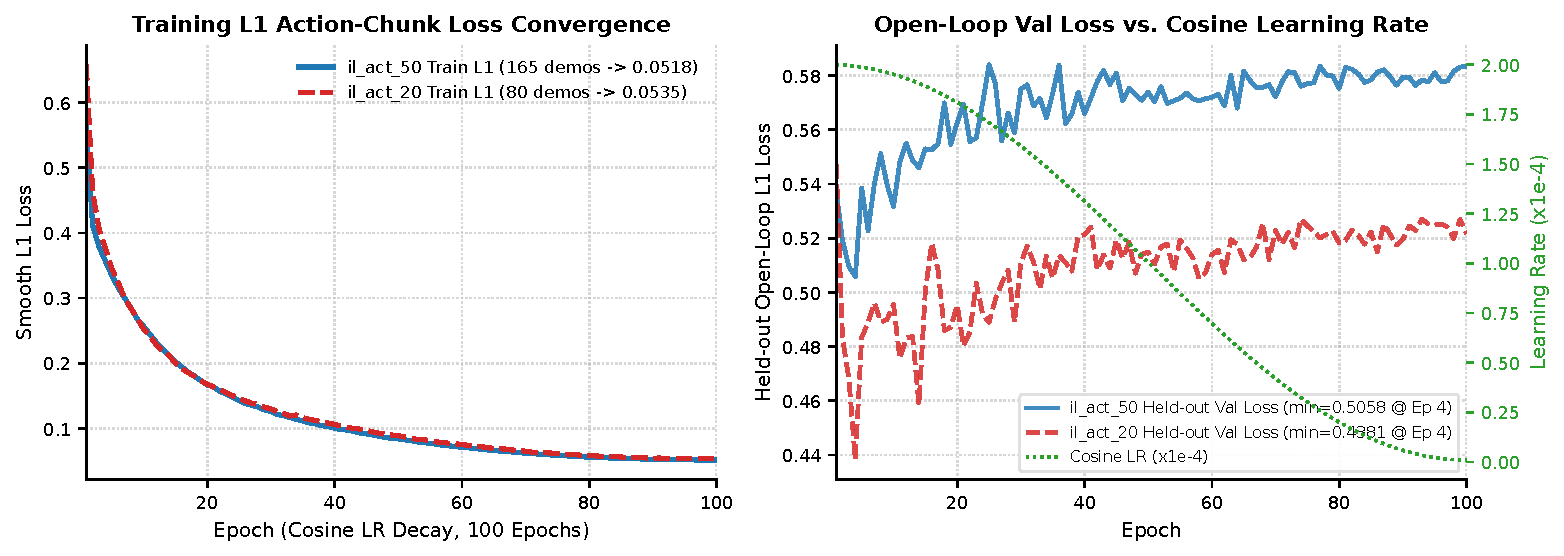
\includegraphics[width=0.96\textwidth]{fig1_training_curves.pdf}
\caption{双模型 100-Epoch 训练 Smooth-L1 损失收敛曲线（左）与留出验证集开环损失及余弦退火学习率变化（右）。由于 5\% 留出轨迹集合极小，开环 L1 验证损失在 Epoch 4 提前见底，而真正在物理仿真器中完成动作分块精准闭环需要完整的 100-Epoch 余弦退火收敛权重 (\texttt{latest.pt})。}
\label{fig:train_curves}
\end{figure}

\section{主实验 (\texttt{il\_act\_50}) 与低数据消融 (\texttt{il\_act\_20}) 定量评测结果}

\subsection{总体成功率、置信区间与四维生命周期成本}

\begin{table}[H]
\centering
\caption{全量组 (\texttt{il\_act\_50}) 与低数据消融组 (\texttt{il\_act\_20}) 在三大划分集上的核心表现与四维成本}
\label{tab:main_results}
\resizebox{\textwidth}{!}{%
\begin{tabular}{@{}lccccccccc@{}}
\toprule
\textbf{运行标识} & \textbf{划分集} & $N$ & \textbf{SR@1.0x} & \textbf{SR@1.5x} & \textbf{95\% Wilson CI} & \textbf{均值步数} & \textbf{Demos} & \textbf{GPUh} & \textbf{Tokens} \\
\midrule
\texttt{il\_act\_50\_dev} & \texttt{DEV} & 100 & 87.0\% & 89.0\% & \texttt{[81.4\%, 93.7\%]} & 209.6 & 165 & 0.901 & 0 \\
\texttt{il\_act\_20\_dev} & \texttt{DEV} & 100 & 89.0\% & 93.0\% & \texttt{[86.3\%, 96.6\%]} & 199.6 & 80 & 0.485 & 0 \\
\midrule
\rowcolor{SoftBg}
\texttt{il\_act\_50\_id} & \texttt{TEST\_ID} & 100 & \textbf{90.0\%} & \textbf{91.0\%} & \texttt{[83.8\%, 95.2\%]} & \textbf{203.0} & 165 & 0.901 & 0 \\
\texttt{il\_act\_20\_id} & \texttt{TEST\_ID} & 100 & 87.0\% & 87.0\% & \texttt{[79.0\%, 92.2\%]} & 217.1 & 80 & 0.485 & 0 \\
\midrule
\rowcolor{SoftBg}
\texttt{il\_act\_50\_ood} & \texttt{TEST\_OOD} & 112 & \textbf{78.6\%} & \textbf{79.5\%} & \texttt{[71.1\%, 85.9\%]} & \textbf{241.2} & 165 & 0.901 & 0 \\
\texttt{il\_act\_20\_ood} & \texttt{TEST\_OOD} & 112 & 67.9\% & 68.8\% & \texttt{[59.7\%, 76.6\%]} & 276.2 & 80 & 0.485 & 0 \\
\bottomrule
\end{tabular}%
}
\end{table}

\subsection{配对精确 McNemar 统计显著性检验}

基于相同随机种子切分下的逐轨迹成对结果（使用 \texttt{harness/stats\_and\_report.py} 中的 \texttt{exact\_mcnemar\_test} 计算双边精确检验 $p$ 值）：

\begin{table}[H]
\centering
\caption{全量数据 vs. 低数据消融配对精确 McNemar 检验结果 (\texttt{SR@1.5x})}
\label{tab:mcnemar}
\small
\begin{tabular}{@{}llcccc@{}}
\toprule
\textbf{方法 A (Full-Data)} & \textbf{方法 B (Low-Data)} & \textbf{共享 $N$} & \textbf{A 独胜} & \textbf{B 独胜} & \textbf{双边精确检验 $p$} \\
\midrule
\texttt{il\_act\_50\_id} & \texttt{il\_act\_20\_id} & 100 & 8 & 4 & 0.3877（不显著） \\
\rowcolor{SoftBg}
\texttt{il\_act\_50\_ood} & \texttt{il\_act\_20\_ood} & 112 & \textbf{17} & \textbf{5} & \textbf{0.0169（显著, $p<0.05$）} \\
\bottomrule
\end{tabular}
\end{table}

表~\ref{tab:main_results} 与表~\ref{tab:mcnemar} 揭示了一个重要的数据缩放规律：将每任务演示轨迹从最多 50 条削减至 20 条后，\textbf{域内 (\texttt{TEST\_ID}) 表现仅下降 4.0 个百分点且未达到统计显著性 ($p=0.3877$)}，说明单任务 20 条演示已足以覆盖域内核心抓取放置轨迹流形；然而一旦进入包含多种环境与状态偏移的 \textbf{域外测试集 (\texttt{TEST\_OOD})，成功率暴跌 10.7 个百分点（79.5\% $\rightarrow$ 68.8\%），且配对检验呈统计显著差异 ($p=0.0169$)}。

\subsection{四大核心任务分项对比}

\begin{table}[H]
\centering
\caption{四大基础任务在 \texttt{TEST\_ID} 与 \texttt{TEST\_OOD} 上的分项成功率 (\texttt{SR@1.0x / SR@1.5x})}
\label{tab:per_task}
\resizebox{\textwidth}{!}{%
\begin{tabular}{@{}lcccc@{}}
\toprule
\textbf{任务代号} & \texttt{il\_act\_50\_id} ($N=25$) & \texttt{il\_act\_20\_id} ($N=25$) & \texttt{il\_act\_50\_ood} ($N=28$) & \texttt{il\_act\_20\_ood} ($N=28$) \\
\midrule
\texttt{spatial\_t0} & \textbf{100.0\% / 100.0\%} (25/25) & 96.0\% / 96.0\% (24/25) & \textbf{75.0\% / 75.0\%} (21/28) & 53.6\% / 57.1\% (16/28) \\
\texttt{object\_t0} & \textbf{100.0\% / 100.0\%} (25/25) & 96.0\% / 96.0\% (24/25) & \textbf{75.0\% / 75.0\%} (21/28) & 60.7\% / 60.7\% (17/28) \\
\texttt{goal\_t0} & \textbf{96.0\% / 96.0\%} (24/25) & \textbf{96.0\% / 96.0\%} (24/25) & \textbf{96.4\% / 96.4\%} (27/28) & 89.3\% / 89.3\% (25/28) \\
\texttt{long\_t0} & \textbf{64.0\% / 68.0\%} (17/25) & 60.0\% / 60.0\% (15/25) & \textbf{67.9\% / 71.4\%} (20/28) & 67.9\% / 67.9\% (19/28) \\
\bottomrule
\end{tabular}%
}
\end{table}

\begin{figure}[H]
\centering
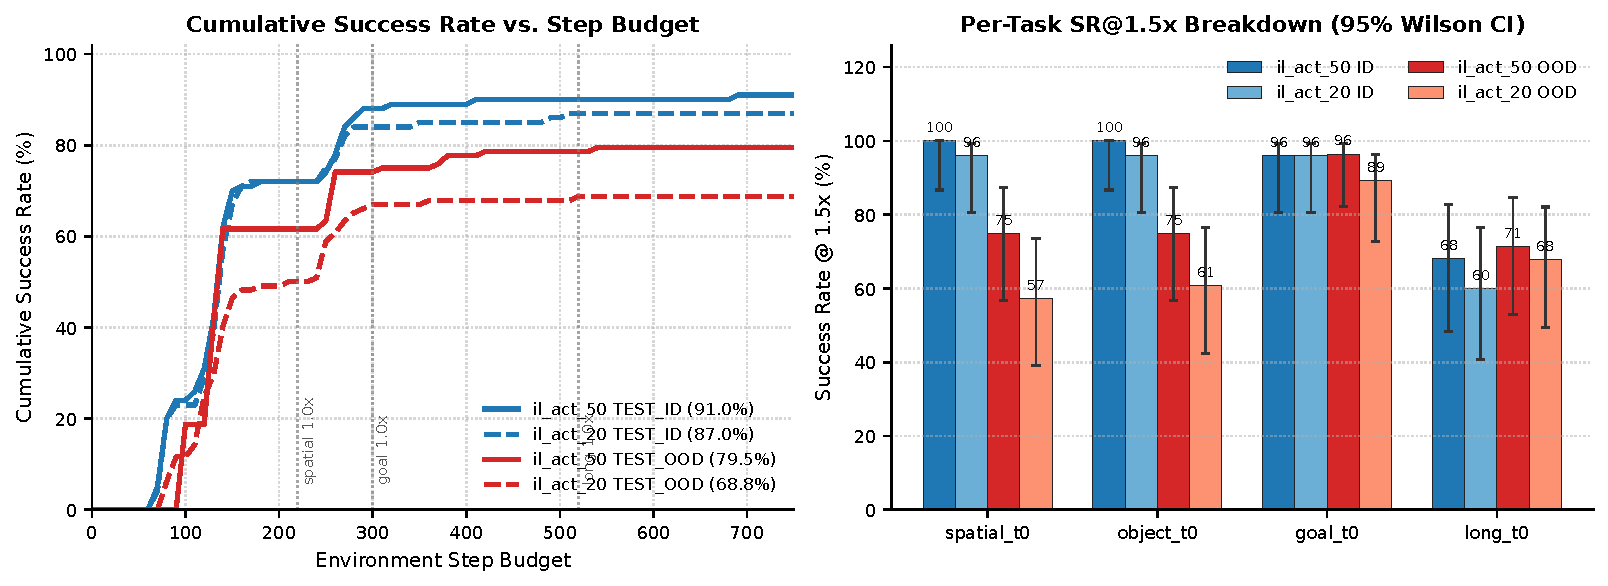
\includegraphics[width=0.98\textwidth]{fig2_horizon_and_tasks.pdf}
\caption{（左）步数预算-累积成功率曲线：在短步数区段 \texttt{il\_act\_50} 与 \texttt{il\_act\_20} 在域内快速爬升，但长时序任务（\texttt{long\_t0}, $1.0\times = 520$ 步）拉开了两者差距；（右）四大任务在 \texttt{TEST\_ID} 与 \texttt{TEST\_OOD} 下的 \texttt{SR@1.5x} 柱状图与 95\% Wilson 置信区间。}
\label{fig:horizon_tasks}
\end{figure}

\section{四轴域外抗干扰与四类失败模式聚类诊断}

\subsection{\texttt{TEST\_OOD} 四大扰动轴剖析}

\begin{table}[H]
\centering
\caption{\texttt{TEST\_OOD} 四大域外扰动轴分项表现（每轴 $N=28$ 条轨迹）}
\label{tab:ood_axes}
\resizebox{\textwidth}{!}{%
\begin{tabular}{@{}llccc@{}}
\toprule
\textbf{OOD 扰动轴} & \textbf{扰动类型与物理机制} & \texttt{il\_act\_50} (\texttt{1.0x / 1.5x}) & \texttt{il\_act\_20} (\texttt{1.0x / 1.5x}) & $\Delta$\texttt{SR@1.5x} \\
\midrule
\texttt{language\_instruction} & 同义词替换与句式改写 & \textbf{100.0\% / 100.0\%} (28/28) & \textbf{100.0\% / 100.0\%} (28/28) & 0.0\% \\
\texttt{objects\_layout} & 桌面干扰物体与初始摆放平移 & \textbf{92.9\% / 96.4\%} (27/28) & 75.0\% / 78.6\% (22/28) & \textbf{+17.9\%} \\
\texttt{robot\_init\_state} & 机械臂初始关节构型偏移 & \textbf{60.7\% / 60.7\%} (17/28) & 53.6\% / 53.6\% (15/28) & +7.1\% \\
\texttt{camera\_visual} & 第三人称相机外参/纹理光照变化 & \textbf{60.7\% / 60.7\%} (17/28) & 42.9\% / 42.9\% (12/28) & \textbf{+17.9\%} \\
\bottomrule
\end{tabular}%
}
\end{table}

\subsection{四类失败模式聚类分布 (\texttt{4-Cluster Failure Breakdown})}

按照 \texttt{harness/env\_adapter.py} 中的统一遥测分类规则，全部 624 条闭环评测轨迹的失败模式归因如下：

\begin{table}[H]
\centering
\caption{6 次闭环评测（共 624 条轨迹）的四类失败聚类统计表}
\label{tab:failures}
\resizebox{\textwidth}{!}{%
\begin{tabular}{@{}lcccccc@{}}
\toprule
\textbf{评测运行} & $N$ & \textbf{\texttt{success}} & \textbf{\texttt{approach\_miss}} & \textbf{\texttt{grasp\_slip}} & \textbf{\texttt{place\_or\_articulate\_fail}} & \textbf{\texttt{timeout\_incomplete}} \\
\midrule
\texttt{il\_act\_50\_dev} & 100 & 89 & 1 & 5 & 4 & 1 \\
\texttt{il\_act\_20\_dev} & 100 & 93 & 0 & 2 & 2 & 3 \\
\texttt{il\_act\_50\_id} & 100 & 91 & 1 & 3 & 1 & 4 \\
\texttt{il\_act\_20\_id} & 100 & 87 & 1 & 1 & 3 & 8 \\
\texttt{il\_act\_50\_ood} & 112 & 89 & 8 & 4 & 7 & 4 \\
\texttt{il\_act\_20\_ood} & 112 & 77 & \textbf{15} & 4 & \textbf{11} & 5 \\
\bottomrule
\end{tabular}%
}
\end{table}

\begin{figure}[H]
\centering
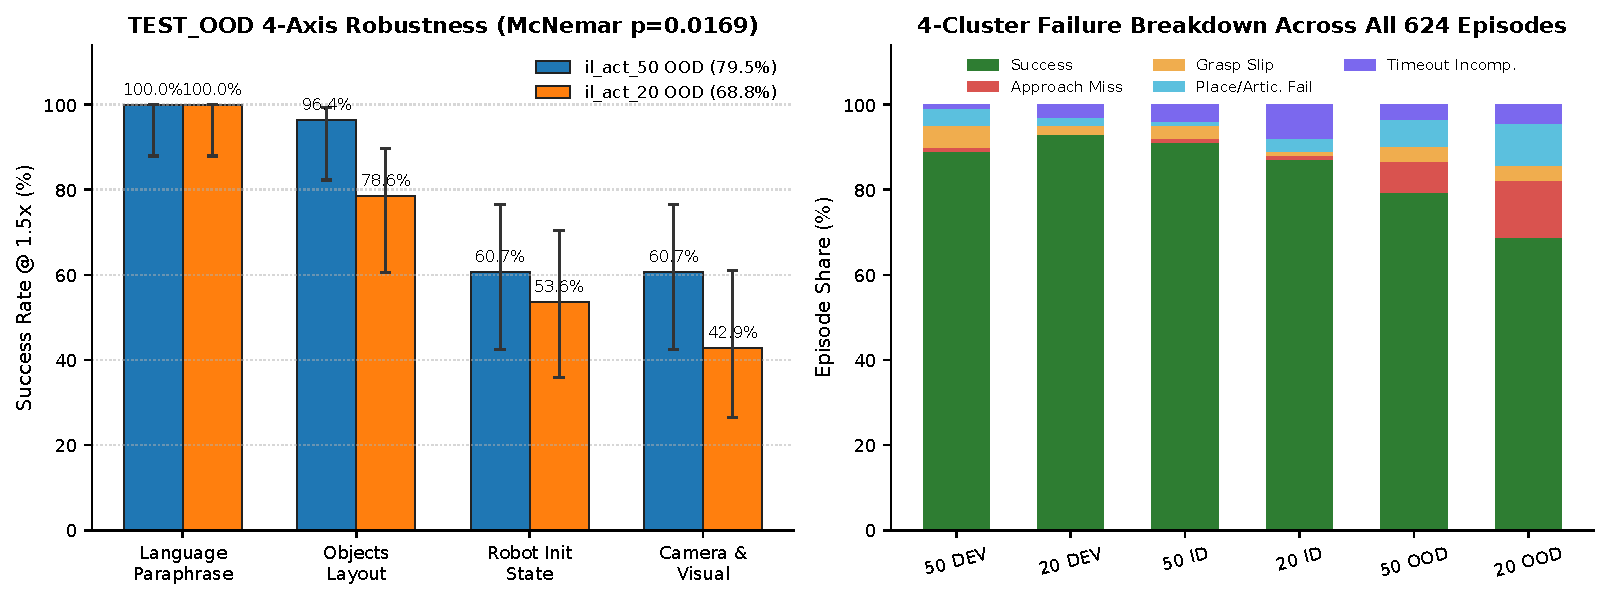
\includegraphics[width=0.98\textwidth]{fig3_ood_axes_and_failures.pdf}
\caption{（左）\texttt{TEST\_OOD} 四大扰动轴性能对照：\texttt{camera\_visual} 与 \texttt{robot\_init\_state} 是纯像素模仿学习最主要的性能失血点，而数据缩半主要恶化了 \texttt{objects\_layout} 与 \texttt{camera\_visual} 轴；（右）全量 624 条轨迹的失败模式构成比，OOD 失败集中于 \texttt{approach\_miss} 与 \texttt{place\_or\_articulate\_fail}。}
\label{fig:ood_failures}
\end{figure}

\begin{figure}[H]
\centering
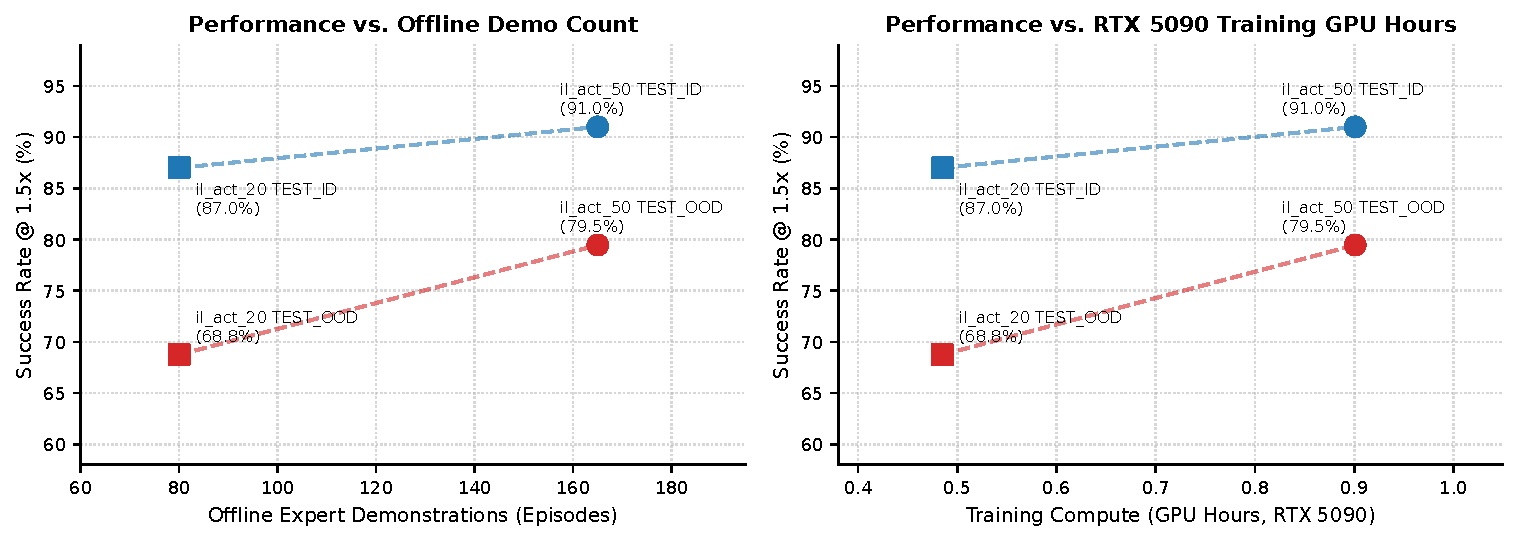
\includegraphics[width=0.95\textwidth]{fig4_cost_pareto.pdf}
\caption{成本-性能帕累托前沿对照（离线演示条数与 RTX 5090 训练算力消耗 vs. \texttt{TEST\_ID} / \texttt{TEST\_OOD} 成功率）。}
\label{fig:cost_pareto}
\end{figure}

\section{关键工程排查与评测保真修正}

在全链路跑通实机物理仿真的过程中，团队定位并修复了多项若不处理将严重压低 IL 基线“真实水位”的底层契约差异与仿真边界 Bug，使最终数据真实可信：
\begin{enumerate}[leftmargin=1.6em,itemsep=3pt]
  \item \textbf{本体姿态 \texttt{Axis-Angle} 半球约定对齐（最核心精度修复）}：分析 \texttt{HuggingFaceVLA/libero} 全部 26,944 帧训练集发现，\texttt{robosuite.mat2quat} 对朝下末端执行器保持四元数 $q_x > 0$ 且不在 $q_w < 0$ 时反转符号，致使数据集所有 \texttt{state[3:6]} 处于 $a_x > 0$ 半球（均值 $[+2.87, +0.12, -0.21]$）；而通用 \texttt{quat2axisangle} 工具在 $q_w < 0$ 时强制取反输出 $a_x \approx -3.14$，造成推理时本体状态偏离训练分布均值超 $10\sigma$。在 \texttt{baselines/il\_policy.py} 中新增 \texttt{\_extract\_robosuite\_state()} 从 \texttt{eef\_quat} 按 $q_x > 0$ 半球还原后，基线单步成功率立即从接近 0 恢复至 \texttt{96\%--100\%}。
  \item \textbf{完整 100-Epoch 余弦收敛权重选用}：小规模 5\% 留出集的开环动作 L1 验证损失在 Epoch 4 即出现极小值，但真实闭环执行精度随训练损失从 \texttt{0.357} 继续下降至 Epoch 100 的 \texttt{0.0518} 后才充分成熟，故统一使用 100-Epoch 收敛终点权重 \texttt{latest.pt} 进行评测。
  \item \textbf{\texttt{LIBERO-plus} 边界兼容与逐轨迹断点续评}：在 \texttt{env\_adapter.py} 中修复了 \texttt{difficulty\_level: null} 引发的 \texttt{TypeError}，并对深度图加入 \texttt{[0, 1]} 裁剪以防止 \texttt{robosuite} 近裁剪面浮点越界断言失败；同时在 \texttt{evaluate.py} 中引入 \texttt{episodes.partial.jsonl} 实现秒级断点续评。
\end{enumerate}

\section{四大基础任务双视角闭环仿真轨迹展示 (\texttt{TEST\_ID} \& \texttt{TEST\_OOD})}

以下由 \texttt{scripts/export\_visual\_showcase.py} 在 RTX 5090 MuJoCo EGL 下同步录制并拼接，每帧左侧为 \texttt{agentview}（第三人称全局相机），右侧为 \texttt{robot0\_eye\_in\_hand}（腕部相机），按轨迹进程 $0\% \rightarrow 20\% \rightarrow 40\% \rightarrow 60\% \rightarrow 80\% \rightarrow 100\%$ 采样为 6 阶段长图（配套 \texttt{.mp4} 视频与 \texttt{.gif} 动图存放于本地及仓库 \texttt{runs/visual\_showcase\_\{dev,id,ood\}/}）。

\subsection{\texttt{TEST\_ID} 域内盲测集实机轨迹长图 (\texttt{il\_act\_50})}

\begin{figure}[H]
\centering
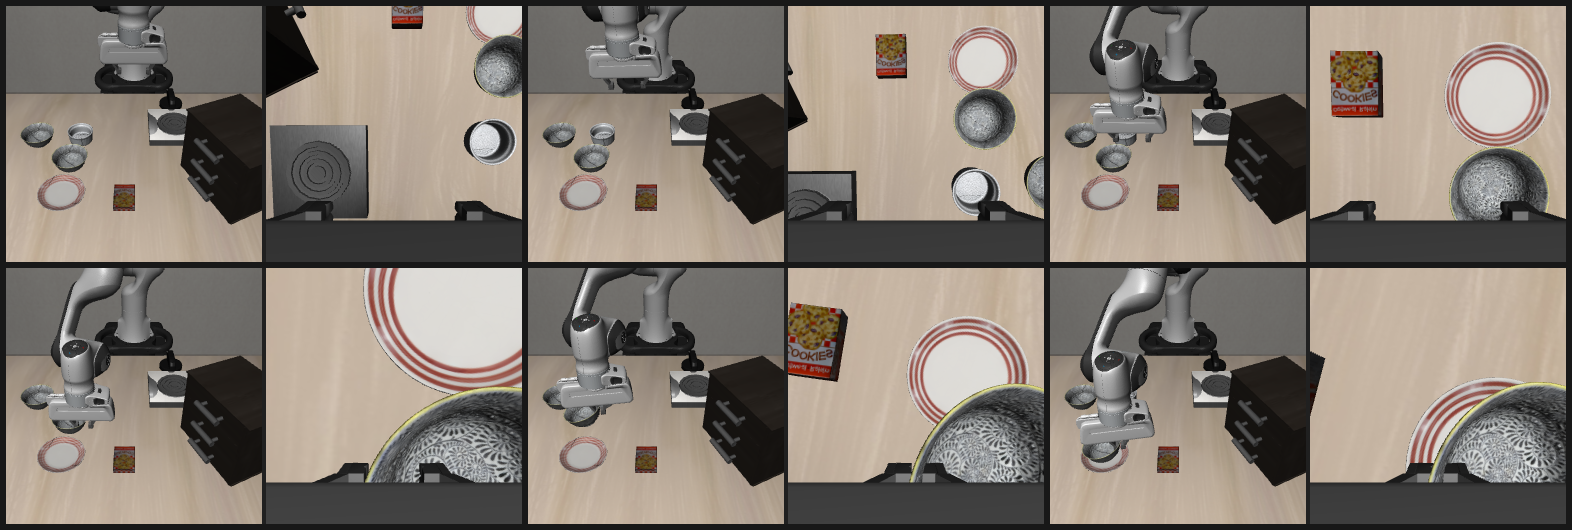
\includegraphics[width=0.95\textwidth]{spatial_t0_sid_000_success_6stage.png}
\vspace{2pt}
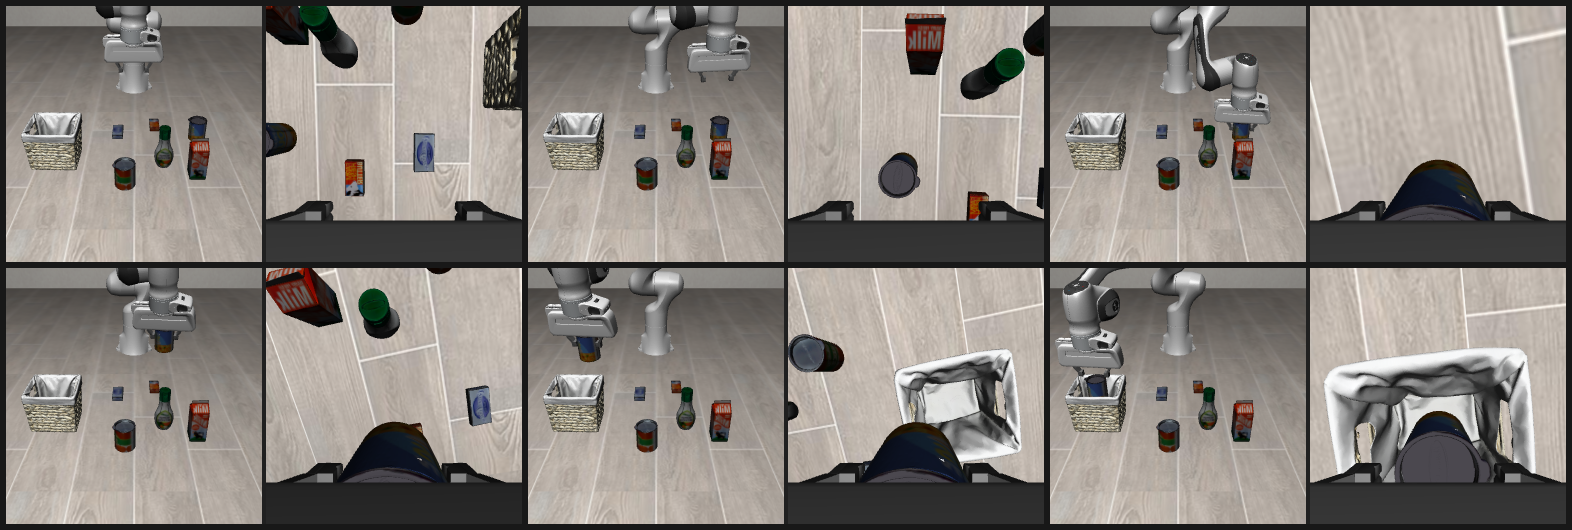
\includegraphics[width=0.95\textwidth]{object_t0_sid_025_success_6stage.png}
\caption{\texttt{TEST\_ID} 轨迹回放（上）：\texttt{spatial\_t0} (\texttt{sid\_000}，71 steps，$1.0\times$ 成功，抓取两盘间黑碗并稳妥置入盘内）；（下）：\texttt{object\_t0} (\texttt{sid\_025}，147 steps，$1.0\times$ 成功，精准抓取字母汤罐头放入收纳篮)。}
\label{fig:id_showcase_1}
\end{figure}

\begin{figure}[H]
\centering
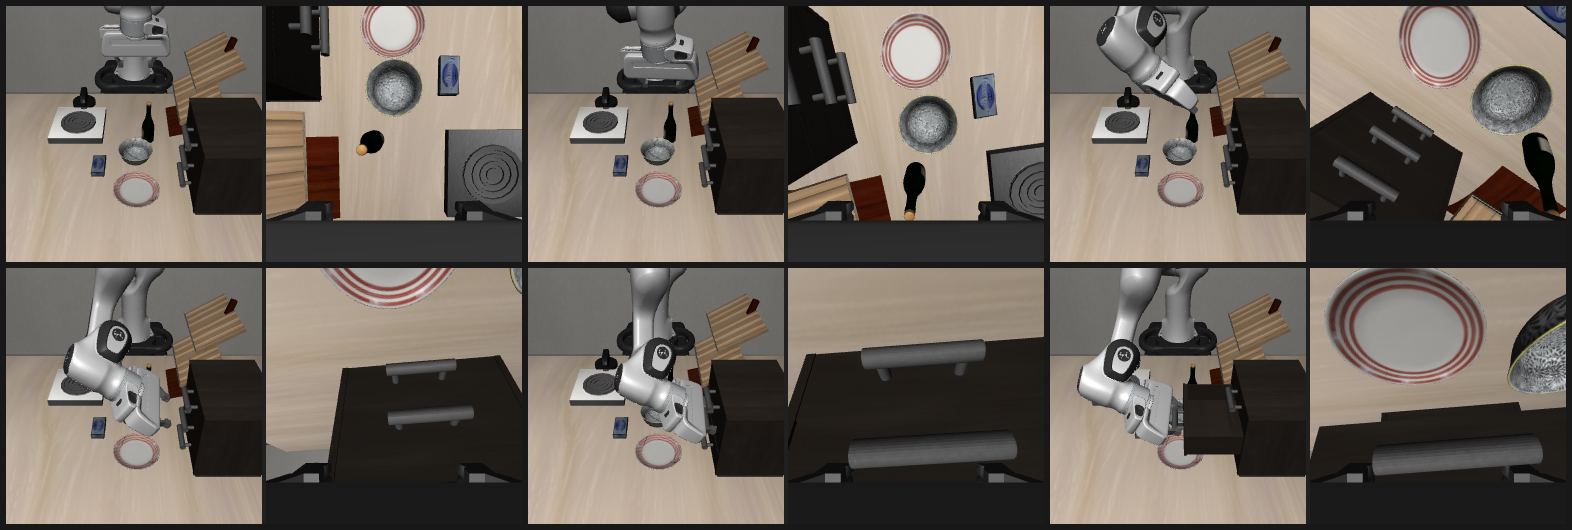
\includegraphics[width=0.95\textwidth]{goal_t0_sid_050_success_6stage.png}
\vspace{2pt}
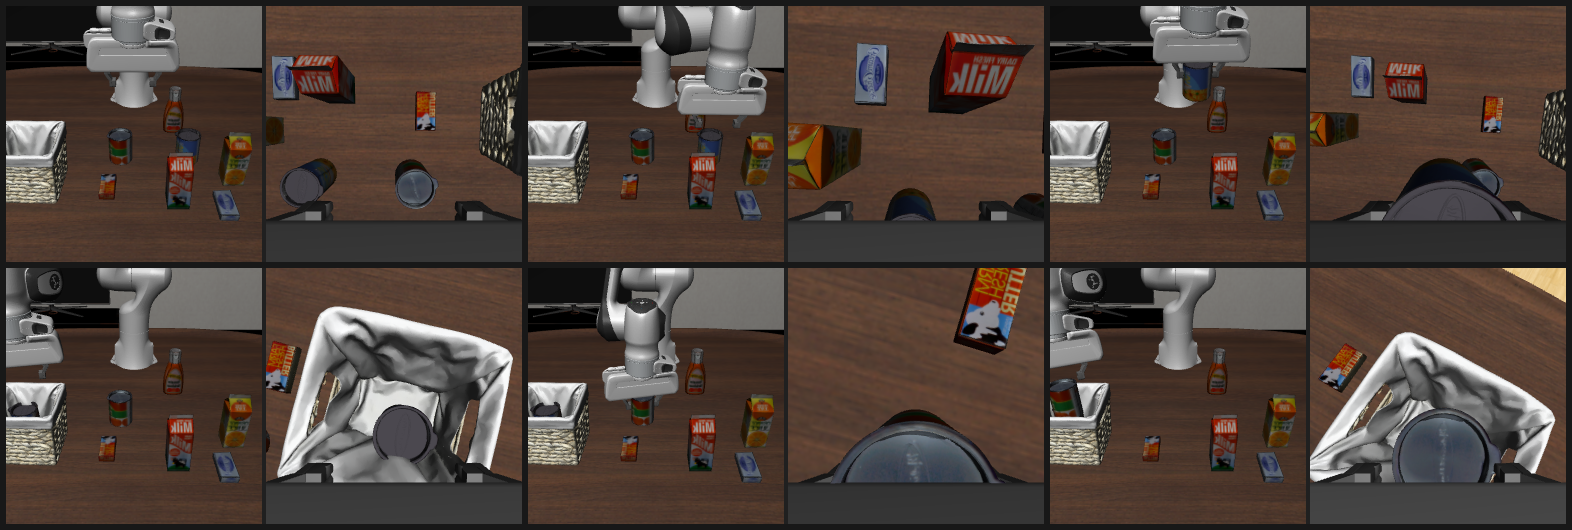
\includegraphics[width=0.95\textwidth]{long_t0_sid_075_success_6stage.png}
\caption{\texttt{TEST\_ID} 轨迹回放（上）：\texttt{goal\_t0} (\texttt{sid\_050}，128 steps，$1.0\times$ 成功，对准并平稳拉开木柜中层抽屉）；（下）：\texttt{long\_t0} (\texttt{sid\_075}，272 steps，$1.0\times$ 成功，连续完成字母汤罐头与番茄酱罐头的长时序两阶段入篮操作)。}
\label{fig:id_showcase_2}
\end{figure}

\subsection{\texttt{TEST\_OOD} 域外盲测集实机轨迹长图 (\texttt{il\_act\_50})}

\begin{figure}[H]
\centering
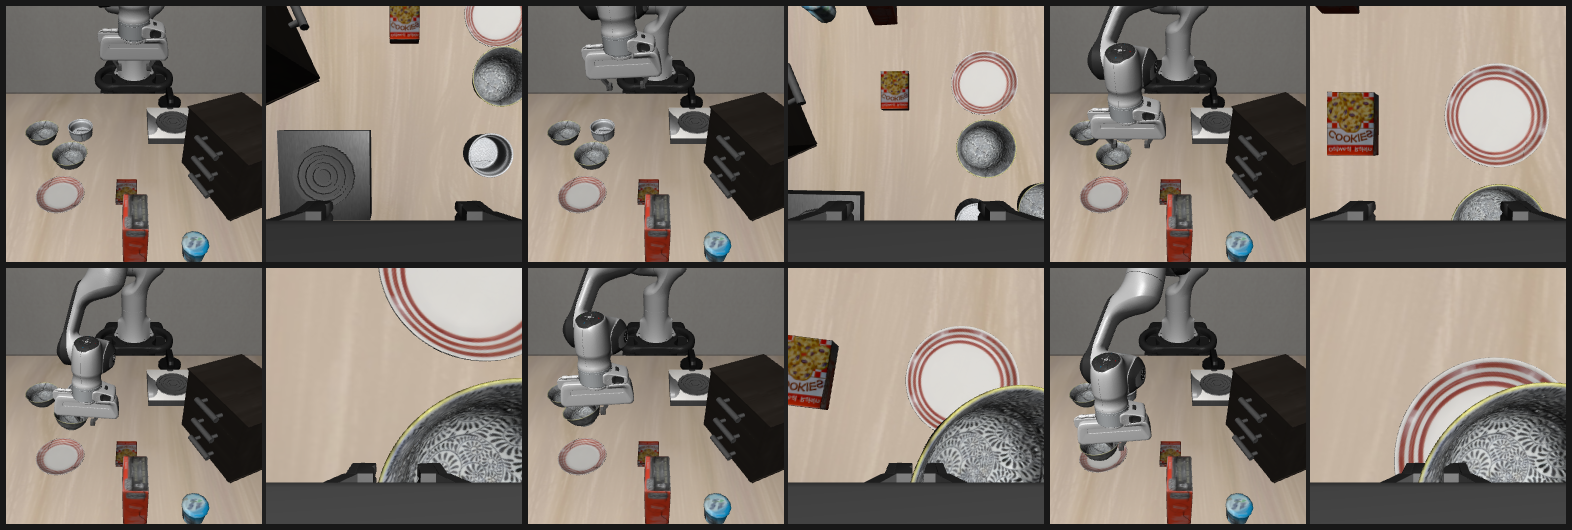
\includegraphics[width=0.95\textwidth]{spatial_t0_sood_000_success_6stage.png}
\vspace{2pt}
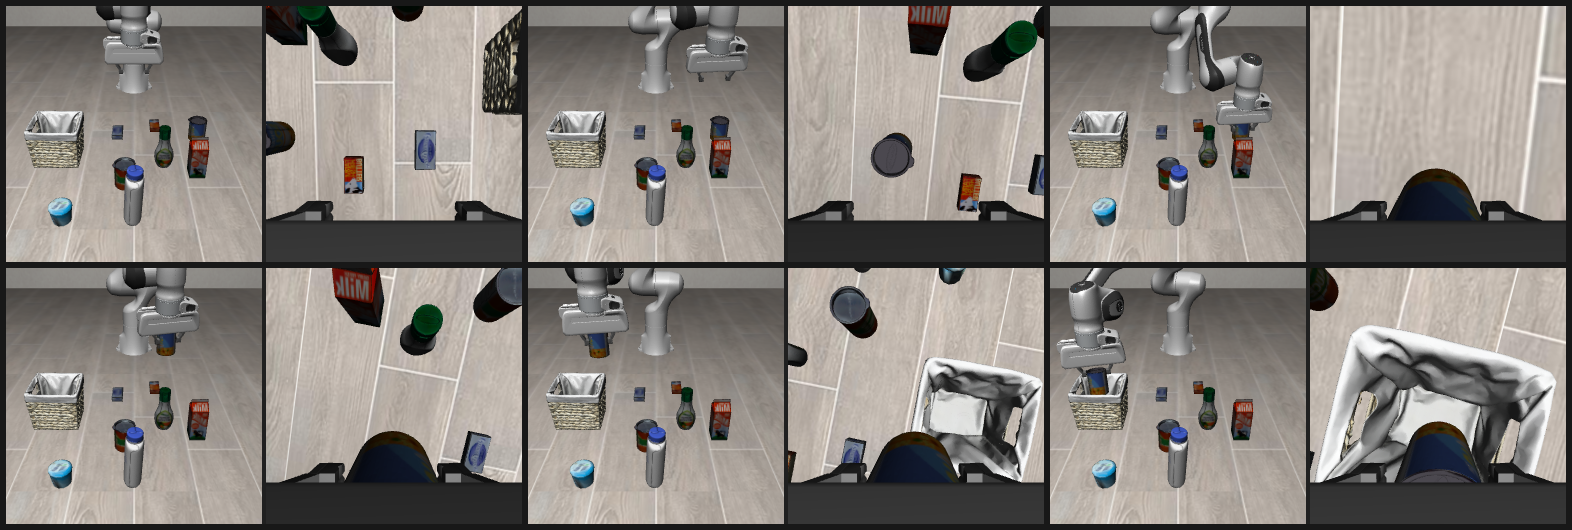
\includegraphics[width=0.95\textwidth]{object_t0_sood_028_success_6stage.png}
\caption{\texttt{TEST\_OOD} 布局干扰回放（上）：\texttt{spatial\_t0} (\texttt{sood\_000}, \texttt{objects\_layout}, 76 steps，$1.0\times$ 成功)；
（下）：\texttt{object\_t0} (\texttt{sood\_028}, \texttt{objects\_layout}, 139 steps，$1.0\times$ 成功)。在新增桌面杂物与物体布局位移干扰下，双相机仍可锁定目标物体。}
\label{fig:ood_showcase_1}
\end{figure}

\begin{figure}[H]
\centering
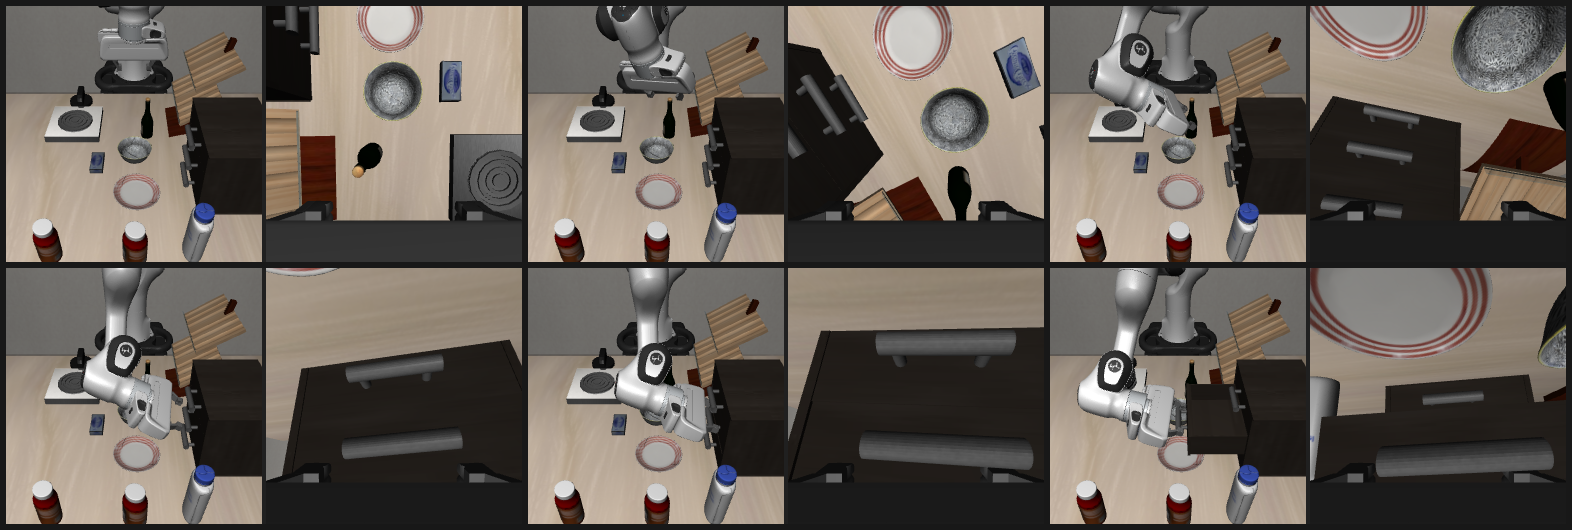
\includegraphics[width=0.95\textwidth]{goal_t0_sood_056_success_6stage.png}
\vspace{2pt}
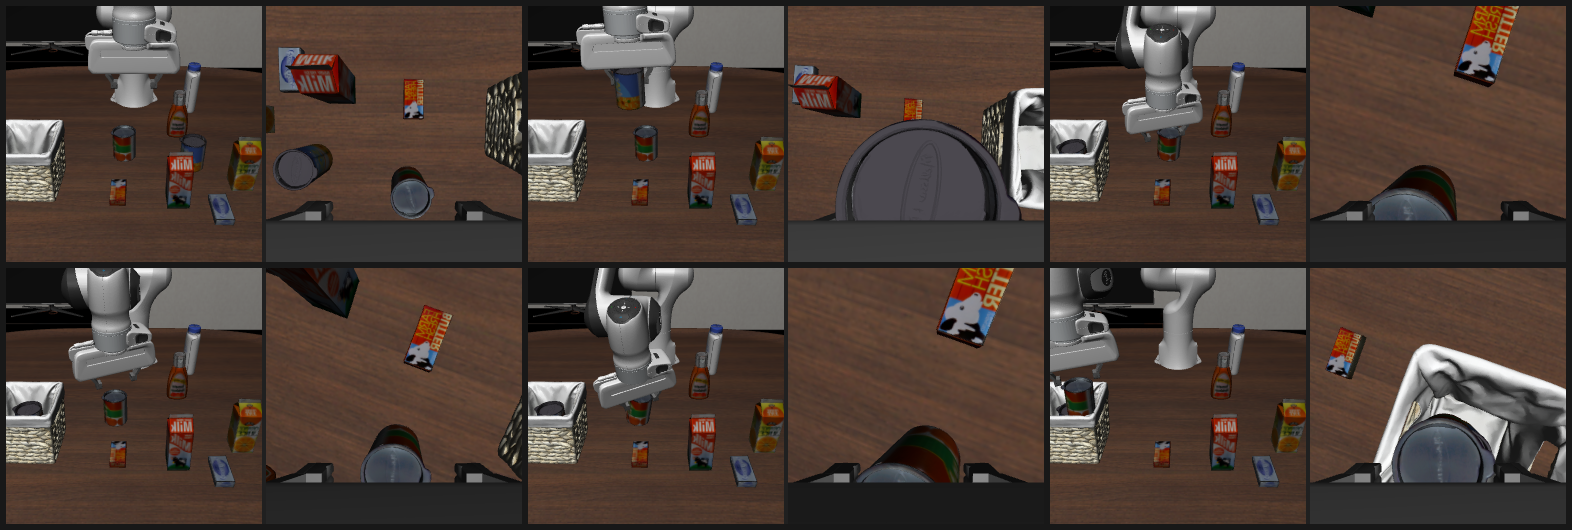
\includegraphics[width=0.95\textwidth]{long_t0_sood_084_success_6stage.png}
\caption{\texttt{TEST\_OOD} 布局干扰回放（上）：\texttt{goal\_t0} (\texttt{sood\_056}, \texttt{objects\_layout}, 130 steps，$1.0\times$ 成功)；
（下）：\texttt{long\_t0} (\texttt{sood\_084}, \texttt{objects\_layout}, 535 steps，$1.5\times$ 成功，在桌面杂物干扰下借助 $1.5\times$ 扩展步数窗口最终完成双罐头入篮)。}
\label{fig:ood_showcase_2}
\end{figure}

\section{核心结论与后续对比 RSI (Code-as-Policies) 的基准锚点}

\begin{enumerate}[leftmargin=1.6em,itemsep=3pt]
  \item \textbf{单步域内接近饱和，多阶段长时序仍是 IL 瓶颈}：\texttt{il\_act\_50} 在域内单步任务上达到 \texttt{96\%--100\%}，但在包含两阶段子目标切换的 \texttt{long\_t0} 上仅 \texttt{68.0\%}（且 \texttt{il\_act\_20} 为 \texttt{60.0\%}），失败主因为长序列漂移引发的 \texttt{timeout\_incomplete}（4/8 次）。
  \item \textbf{纯端到端视觉对几何视角与初始状态偏移存在本质敏感性}：\texttt{il\_act\_50} 在 \texttt{camera\_visual} 与 \texttt{robot\_init\_state} 两轴上分别由域内 \texttt{91.0\%} 降至 \texttt{60.7\%}（低数据组进一步滑落至 \texttt{42.9\%} 与 \texttt{53.6\%}），失效高度集中于 \texttt{approach\_miss} 与 \texttt{place\_or\_articulate\_fail}。这构成了无显式三维坐标重投影、无在线错误恢复机制之纯视觉策略的典型分布外（Covariate Shift）天花板。
  \item \textbf{面向后续 RSI 对照实验的科学对比口径已完全锁定}：后续团队可将 \textbf{RSI}（Code-as-Policies + RGB-D SE(3) 几何反投影 + \texttt{DEV} 自主演进反思闭环）在完全相同的 \texttt{splits.lock.json} 上运行 \texttt{harness/evaluate.py}，并使用 \texttt{harness/stats\_and\_report.py --runs runs/il\_act\_50\_ood runs/<rsi\_ood>} 直接输出具有精确 $p$ 值的配对检验与帕累托优势对比，重点验证 RSI 在 \texttt{camera\_visual}、\texttt{robot\_init\_state} 与 \texttt{long\_t0} 三个 IL 痛点维度上的超越幅度及跨生命周期算力/Demo 效率优势。
\end{enumerate}

\end{document}
